% Document Definition
\documentclass[twocolumn]{article}
\usepackage[letterpaper, left=1in, right=1in, top=1in, bottom=1in]{geometry}
\usepackage{amscd,amssymb,amsmath,amsthm,mathtools}
\usepackage{kpfonts}
\usepackage{titling}
\usepackage[
  citestyle=ieee,
  style=ieee
]{biblatex}
\usepackage{listings}
\usepackage{hyperref}

\addbibresource{citations.bib}

\renewcommand{\baselinestretch}{1.1}
\pagenumbering{gobble}

\setlength{\droptitle}{-4em}
\title{\Large\textbf{Determining a Cache Hit/Miss over RDMA -- A NetCAT Replication} \\
CS6465 -- Final Project}
\author{Emerson Ford\hspace{20pt}Calvin Lee}
\posttitle{\par\end{center}}
\predate{}
\postdate{}
\date{}

\begin{document}
\maketitle
\section{Overview}
Timing-based cache side-channels have been a well documented threat since at least 2005 \cite{osvik2006cache}.
By measuring access times to a specific line of memory one can determine with reasonably high accuracy if the access was a cache hit or miss.
Research have shown that this can be used by attackers to recover anything from bits of RSA secret keys to passwords received over the network \cite{schwarz2018keydrown} \cite{yarom2014flush+}.
While further research has shown these types of side channels can bypass even VM isolation boundaries, it appeared these attacks were locally restricted to a host \cite{liu2015last}.
Recently, however, technologies such as Infiniband and DDIO have enabled sub-microsecond remote memory accesses with RDMA and given NICs access to a portion of the last-level cache.
In 2019, VUSec claimed these technologies enable cache side-channels to be accessible through the network. They further claim they were able to use these to perform a remote SSH keystroke timing attack \cite{kurth_netcat:_2020}. We seek to replicate their remote cache side-channel access results which is the basis to enable the rest of the paper. In particular, we wanted to replicate figure \ref{fig:replication_graph}.


% \subsection{RDMA/DDIO Overview}
% Simplified, RDMA enables remote memory accesses without CPU interaction.
% Both the server and client register a portion of memory to be used for RDMA with the NIC.
% The client can then post \texttt{ibverbs} to an in-memory work queue to make read or write requests to a specific remote address in the server's registered memory.
% The NIC polls on this work queue and fulfills the request.
% On a read, the NIC puts the read contents into the client's registered memory.
% On a write, the NIC puts the contents of the client's registered memory at the specified remote address.
% The NIC will then publish a completion message to an in-memory completion queue the client can poll on.
%
% DDIO enables these reads to be served out of LLC if present and enables writes to be placed in LLC as opposed to directly to main memory.
% RDMA reads will not load data into the LLC if it is not present but RDMA writes will.
% DDIO is limited to use a small subset of cache ways \cite{intelddio}.

\subsection{Test Hardware}
We used the following hardware in our experiments:
\begin{enumerate}
 \item Cloudlab Apt Cluster \texttt{r320}: 1 x Xeon E5-2450 processor (8 cores, 2.1Ghz), 16GB Memory (4 x 2GB RDIMMs, 1.6Ghz), 1 x Mellanox MX354A Dual port FDR CX3 adapter w/1 x QSA adapter
 \item Cloudlab Apt Cluster \texttt{c6220}: 2 x Xeon E5-2650v2 processors (8 cores each, 2.6Ghz), 64GB Memory (8 x 8GB DDR-3 RDIMMs, 1.86Ghz), 1 x Mellanox FDR CX3 Single port mezz card
 \item University of Utah Notchpeak Cluster \texttt{notch008}/\texttt{notch010}: 2 x Intel(R) Xeon(R) Gold 6130 CPU @ 2.10GHz, 186GB Memory, EDR Infiniband
\end{enumerate}
As a rough benchmark, on the \texttt{r320}s an \texttt{ib\_read\_lat} took 1900ns on average with 50ns of standard deviation.

\begin{figure}
 \centering
 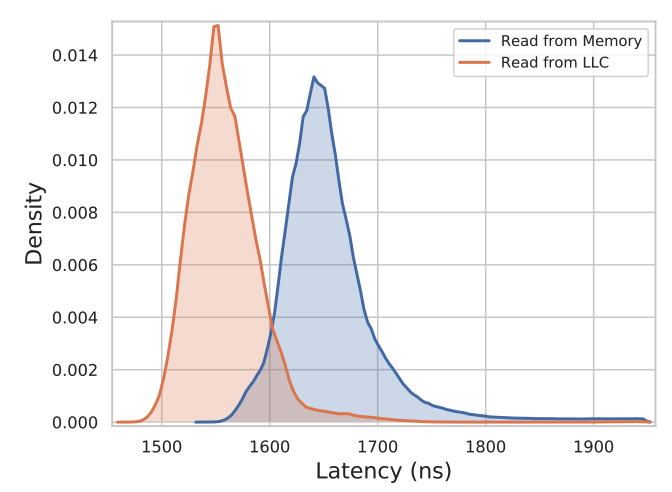
\includegraphics[width=0.40\textwidth]{replication_graph.png}
 \label{fig:replication_graph}
 \caption{Read Timings from the Paper}
\end{figure}

\section{Code}
\subsection{Timing}
On a given remote memory address $x$, we:
\begin{enumerate}
 \item RDMA Read $x$ (cache miss)
 \item RDMA Write to $x$ (pull into cache)
 \item RDMA Read $x$ (cache hit)
\end{enumerate}
and timed the first read and second read.
The following code was used for timing:

\begin{lstlisting}[frame=single,language=C,basicstyle=\footnotesize]
start_cycle_count = start_tsc();

rc = ibv_post_send(res->qp, &sr, &bad_wr);
if (rc)
    fprintf(stderr, "failed to post SR\n");
do {
    poll_result = ibv_poll_cq(res->cq, 1, &wc);
} while (poll_result == 0);

end_cycle_count = stop_tsc();
\end{lstlisting}
Where \texttt{start\_tsc} is an lfence, rdtsc, lfence and \texttt{stop\_tsc} is an rdtscp, lfence.

\subsection{Read$\rightarrow$Write$\rightarrow$Read Methods}
We were uncertain if RDMA writes triggered any cache prefetching.
As such, we developed multiple ways to measure the read$\rightarrow$write$\rightarrow$read operations to overcome any potential prefetching.
\begin{enumerate}
 \item Read-write-read a single address with a \texttt{clflush} between each iteration
 \item Random access across an array, avoiding the cache line hit from the last iteration
 \item Sequential access across an array with strides to (hopefully) overcome any prefetchers (64 byte msgs, columns count = 4, row count = 524288, {\raise.17ex\hbox{$\scriptstyle\mathtt{\sim}$}}134 MB total)
\end{enumerate}

All of our code is available publicly at \url{https://github.com/emersonford/NetCAT-Replication}.

\section{Results}
Please see the presentation for graphs on each method.
\subsection{\texttt{clflush} Method}
Initially, we got seemingly impressive results from the \texttt{clflush} method with a clear separation between the two distributions -- more so than figure \ref{fig:replication_graph}.
However, upon further investigation we found these timings are likely misleading.
A read$\rightarrow$read produced similar results as read$\rightarrow$write$\rightarrow$read albeit with a smaller distance between the two distributions.
We expect it to produce two identical distributions.

We suspect two things may cause this.
First, we use TCP socket communication to synchronize between the server and client.
These result in syscalls that may result in page tables switches, cache evictions, etc that could cause timing anomalies.
Second, there is little documention or research on the pathological behaviors of DDIO.
It is possible there may be side effects from an interaction between DDIO and \texttt{clflush} that cause these timing anomalies.

Ultimately, we ruled this method out for reproducing figure \ref{fig:replication_graph}.

\subsection{Random Access Method}
The data from random access also seemed promising at first.
There appeared to be little noise and the graphs produced lined up closely with figure \ref{fig:replication_graph}.
However, further iterations produced unexpected results, such as the first reads being faster than the second reads.
We suspect this might stems from mistuning of our random access parameters and it may be something we can fix in the future.
However, we also ruled this method out for reproducing figure \ref{fig:replication_graph}.

\subsection{Sequential Access Method}
The data obtained from sequential access consistently gave us expected results, albeit noiser than data from the random access method.
The graphs generated seemed to line up with results from figure \ref{fig:replication_graph}, aside from a few odd timing anomalies as seen in figure \ref{fig:seq_access}.
Furthermore, read$\rightarrow$read produces expected results with sequential access.
Further investigations and improvements to the sequential access method are necessary to clean up data and account for timing anonamlies, but tenatively the data suggests the cache timing results are reproducable.

\begin{figure}
 \centering
 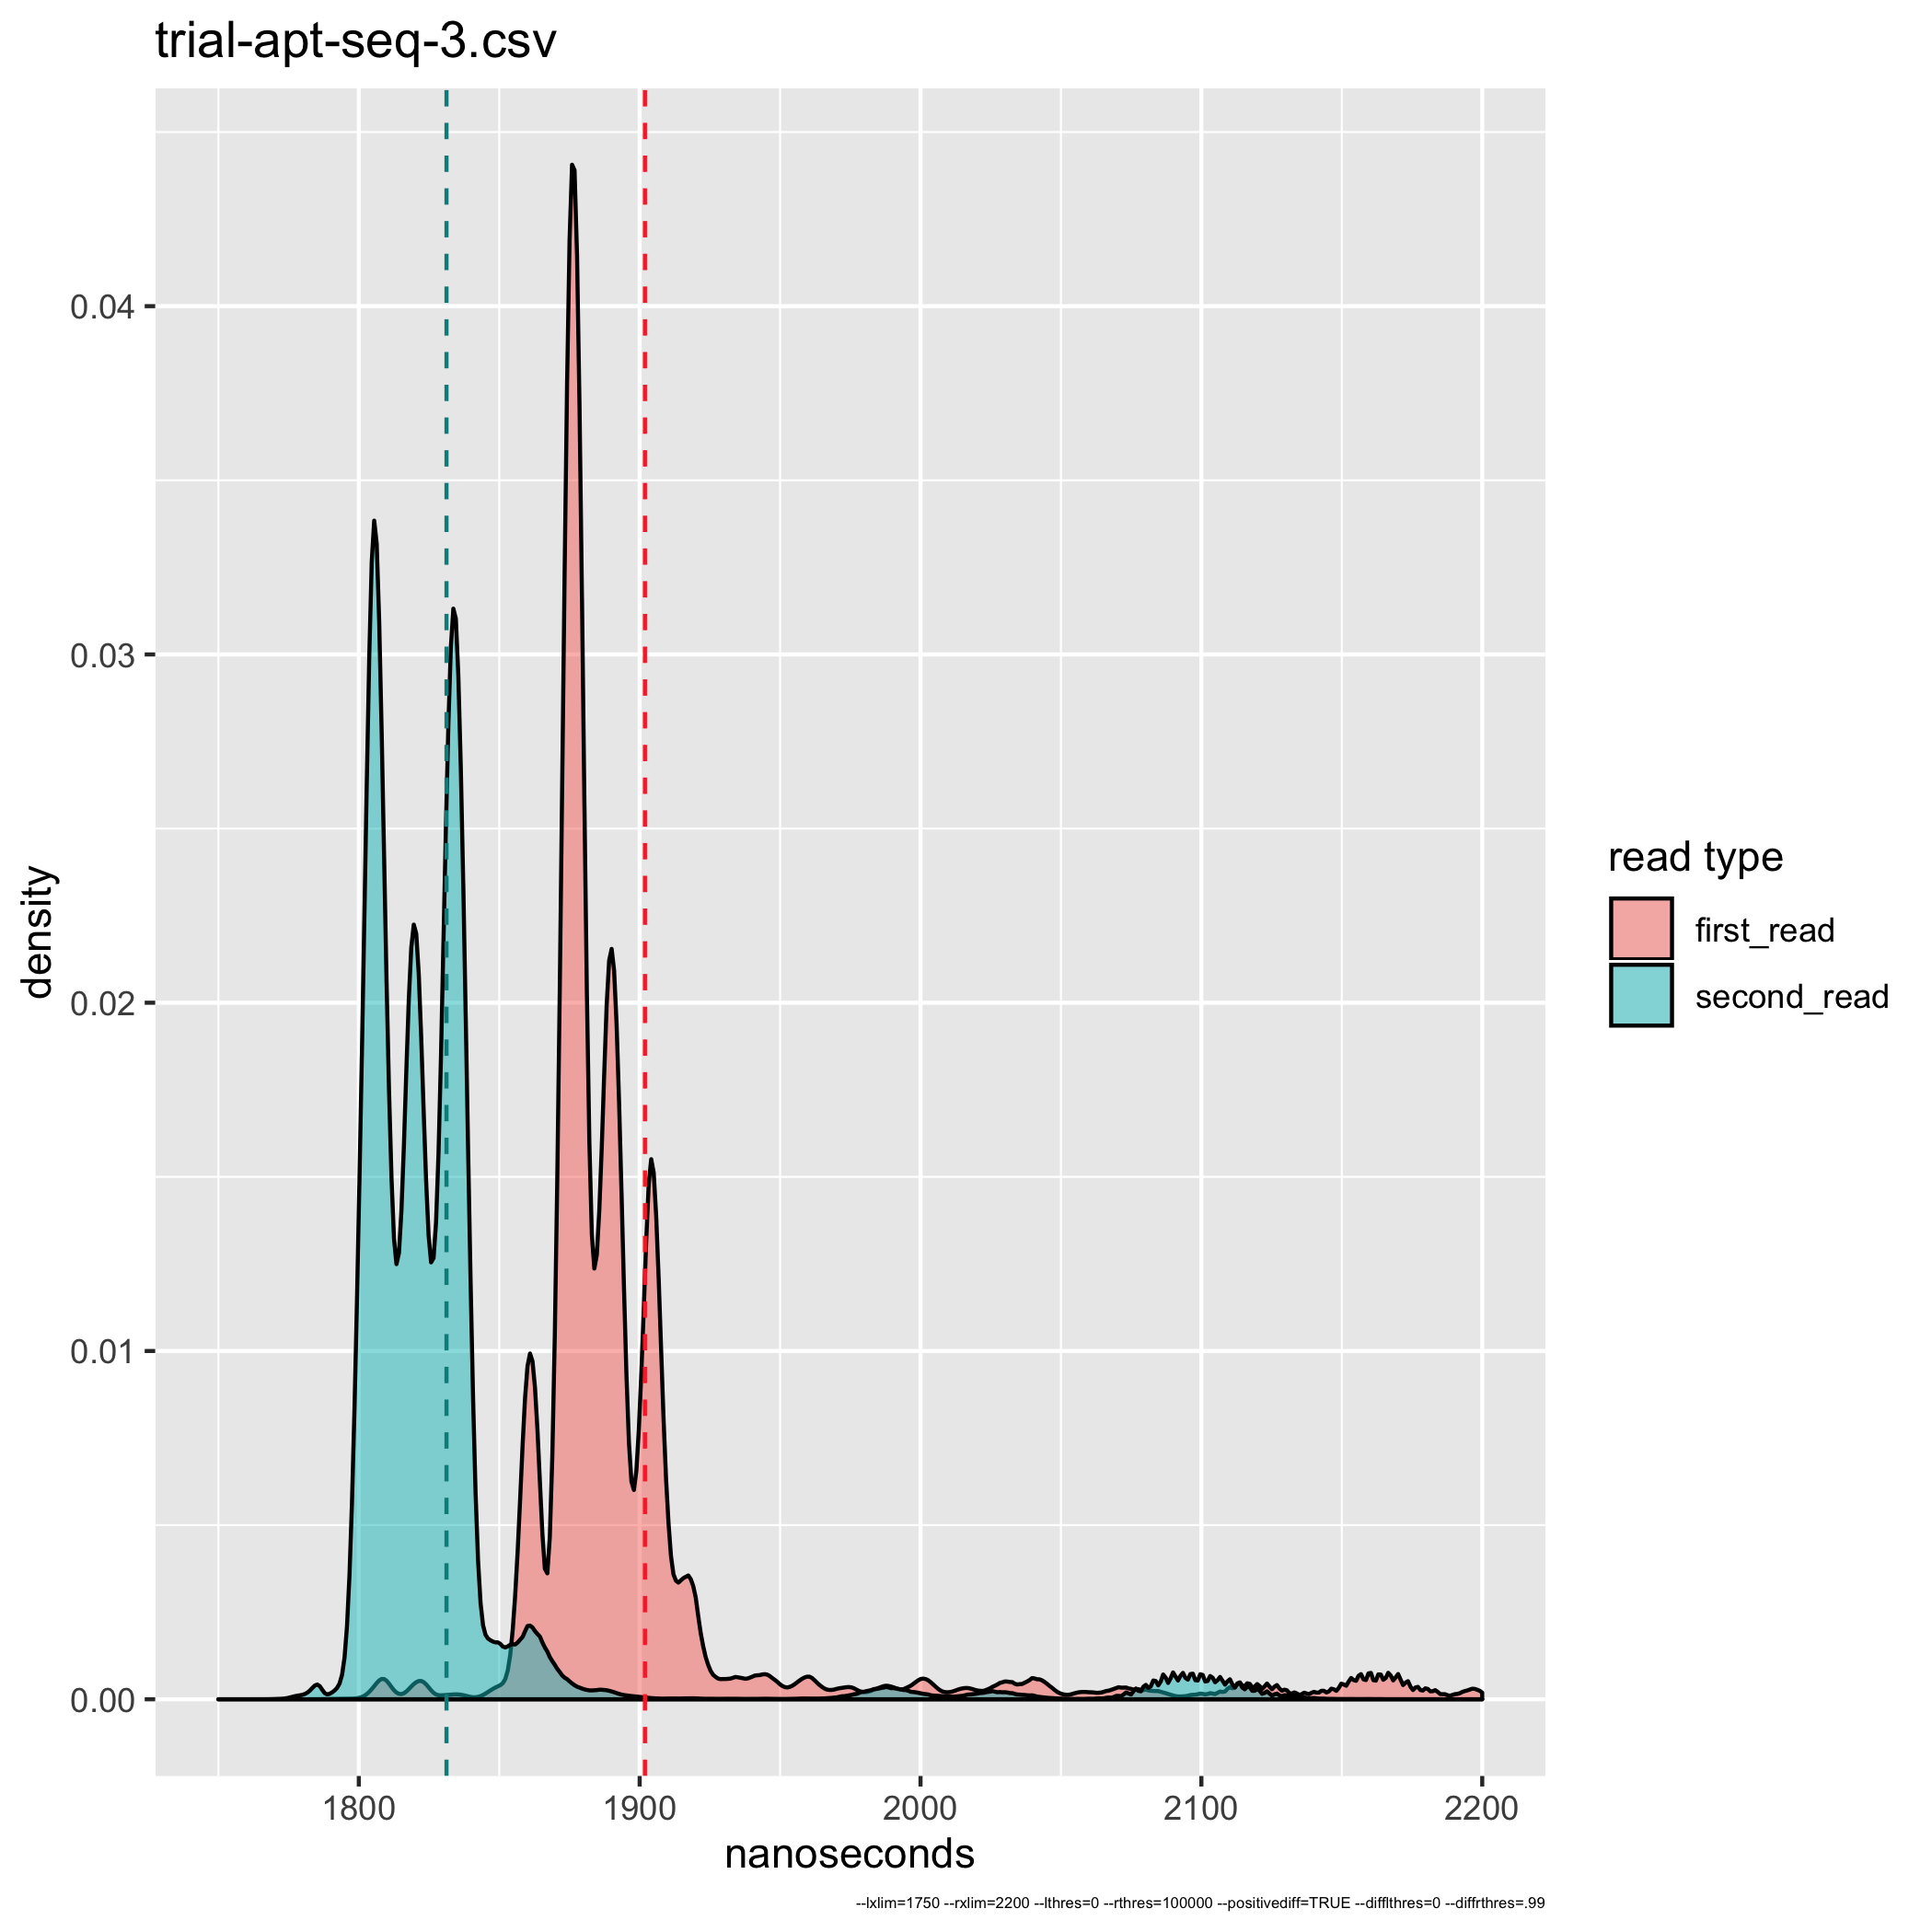
\includegraphics[width=.40\textwidth]{trial-apt-seq-3-histogram.png}
 \caption{Results from a Run of the Sequential Access}
 \label{fig:seq_access}
\end{figure}


\section{Challenges}
We quickly found that timing at a nanosecond granularity is unexpectedly difficult on modern systems.
There are a number of factors that can influence the timing results and there is little documentation for how some parts of the system interact, such as DDIO and the NIC.
Some of the challenges we faced and tried to investigate are:
\subsection{Server Challenges}
\begin{enumerate}
 \item \textbf{NUMA}: it's possible the server's registered memory could be placed in a separate NUMA node than the NIC.
       This would affect timing results as main memory access would then also have to traverse the CPU fabric.
       We investigated how to put our registered memory in the correct NUMA node and what effects incorrect NUMA placement had on our timing.
 \item \textbf{Prefetching}: it's likely there is some prefetching into cache done with an RDMA write, but we were unable to verify this with either data or documentation.
       If the prefetcher is smarter than we expect, it may severly interfere with timing. Further investigations of this are necessary.
 \item \textbf{DDIO Pathologies}: we're uncertain what caused the misleading data from our \texttt{clflush} method.
       It is possible there may be some unexpected interaction with DDIO when \texttt{clflush} is used.
       Further testing of this is required.
 \item \textbf{DDIO Ways Restriction}: DDIO, on Intel Xeon E5 CPUs, is restricted to only 2 of the 20 cache ways in the LLC.
       This limits the types of data we wish to PRIME+PROBE on.
\end{enumerate}

\subsection{Client Challenges}
\begin{enumerate}
 \item \textbf{CPU Frequency/Power Management}: we frequently found the client CPU to dramatic alter in its frequency.
       We're unsure if this contributed to the noise in our data and investigated ways to turn off frequency scaling for our tests to be on the safe side.
       We ended up learning quite a bit about how Intel manages CPU frequencies and the different power states a CPU can be in to solve this.
\end{enumerate}

\subsection{Network Fabric Challenges}
\begin{enumerate}
 \item \textbf{Infiniband Saturation}: it appears the more saturated an Infiniband fabric is, the higher the mean and variance for RDMA read latencies.
       This causes significant issues as the saturation of an Infiniband fabric is difficult to determine. In future tests, we may try to find a non-used Infiniband fabric to control for this.
\end{enumerate}

There are still quite a number of graph anomalies we cannot reason about.
These anomalies make it extremely difficult to do any statistical prediction on whether a read was a cache hit or miss.
Further testing is required to account for these anomalies.

\section{Next Steps}
Continuing on the project, the next steps would be:
\begin{itemize}
 \item Clean up data and reduce data anomalies
 \item Develop a statistical prediction on whether an RDMA read is a cache hit or miss
 \item Use this prediction to build an evicition set on the remote host
 \item Perform a PRIME+PROBE attack on the remote host
\end{itemize}
We suspect each task will be non-trivial based on papers that achieve these locally.

\section{Conclusion}
It appears it is likely one can determine if a remote memory access is served from LLC or main memory, but our data is not conclusive. While we may not have been able to replicate their cache timing results exactly, we did learn quite a bit about the various technologies that go into this paper. Given more time, we feel we could overcome or at least account for these challenges and fully develop a remote PRIME+PROBE attack on a remote host.

\printbibliography
\end{document}
